%! TeX program = xelatex
%! TeX TS-program = xelatex
\documentclass[10pt,dvipsnames]{beamer}
\usepackage{fontspec}
\setmainfont{QTBookmann}
\setsansfont{QTFrizQuad}
\setmonofont[
]{BigBlueTermPlus Nerd Font}
\usepackage{polyglossia}
\usepackage[dvipsnames]{xcolor}
\usepackage{dirtytalk}
\usepackage{graphicx}
\setdefaultlanguage{english}
\usepackage{multirow}
\usepackage{listings}
\usepackage{ragged2e}
\usepackage{listings}
\usepackage{hyperref}
\usepackage[most]{tcolorbox}
\usepackage[backend=biber]{biblatex}
\usetheme{Copenhagen}
\tcbuselibrary{breakable,skins}
%! TeX program = xelatex
%! TeX TS-program = xelatex
%! TeX root = ProgramaciónEvolutiva.tex
%%%%%%%%%%%%%%%%%%%%%%%%%%%%%%%%%%%%%%%%%%%%%%%%%%%%%%%%%%%%%%%%%%%%%%%%
% Define AntiqueWhite color
\definecolor{AntiqueWhite}{RGB}{250,235,215}
\definecolor{mypurple}{RGB}{104,020,108}
\setbeamercolor*{palette primary}{use=structure,fg=white,bg=mypurple}
\setbeamercolor{normal text}{fg=white, bg=black}
\setbeamercolor{tcolorbox text}{fg=white, bg=black}
\setbeamertemplate{navigation symbols}{}                              %
\newcommand{\colouredcircle}{%
  \tikz{\useasboundingbox (-0.2em,-0.32em) rectangle(0.2em,0.32em);
        \draw[ball color=PineGreen!7!Plum!90!Red,shading=ball,line width=0.03em] (0,0) circle(0.18em);}}
\newcommand{\colouredcircledis}{%
  \tikz{\useasboundingbox (-0.2em,-0.32em) rectangle(0.2em,0.32em);
        \draw[ball color=PineGreen!7!Plum!20!Black,shading=ball,line width=0.03em] (0,0) circle(0.18em);}}
\setbeamertemplate{itemize item}{\colouredcircle}
\setbeamercolor*{bibliography entry title}{fg=Yellow!80!White, bg=Black}
% Set beamer bibliography titles and numbers color to antique white
\setbeamercolor*{bibliography entry author}{fg=AntiqueWhite}
\setbeamercolor*{bibliography entry location}{fg=AntiqueWhite}
\setbeamercolor*{bibliography entry note}{fg=AntiqueWhite}
%% Numbering color to Pine Green
\setbeamercolor*{bibliography item}{fg=LimeGreen!80!White}
% Set beamer bibliography urls color to some magenta
\setbeamercolor*{bibliography entry url}{fg=Magenta}
% Captions color to rgba (0,255,0,1)
\definecolor{LimeGreen}{RGB}{0,255,0}
\setbeamercolor{caption name}{fg=LimeGreen}
%%%%%%%%%%%%%%%%%%%%%%%%%%%%%%%%%%%%%%%%%%%%%%%%%%%%%%%%%%%%%%%%%%%%%%%%
\usepackage{tikzpagenodes}
\setbeamertemplate{background canvas}{%
  \begin{tikzpicture}[inner sep=0pt,remember picture,overlay]
    \node at (current page.center) {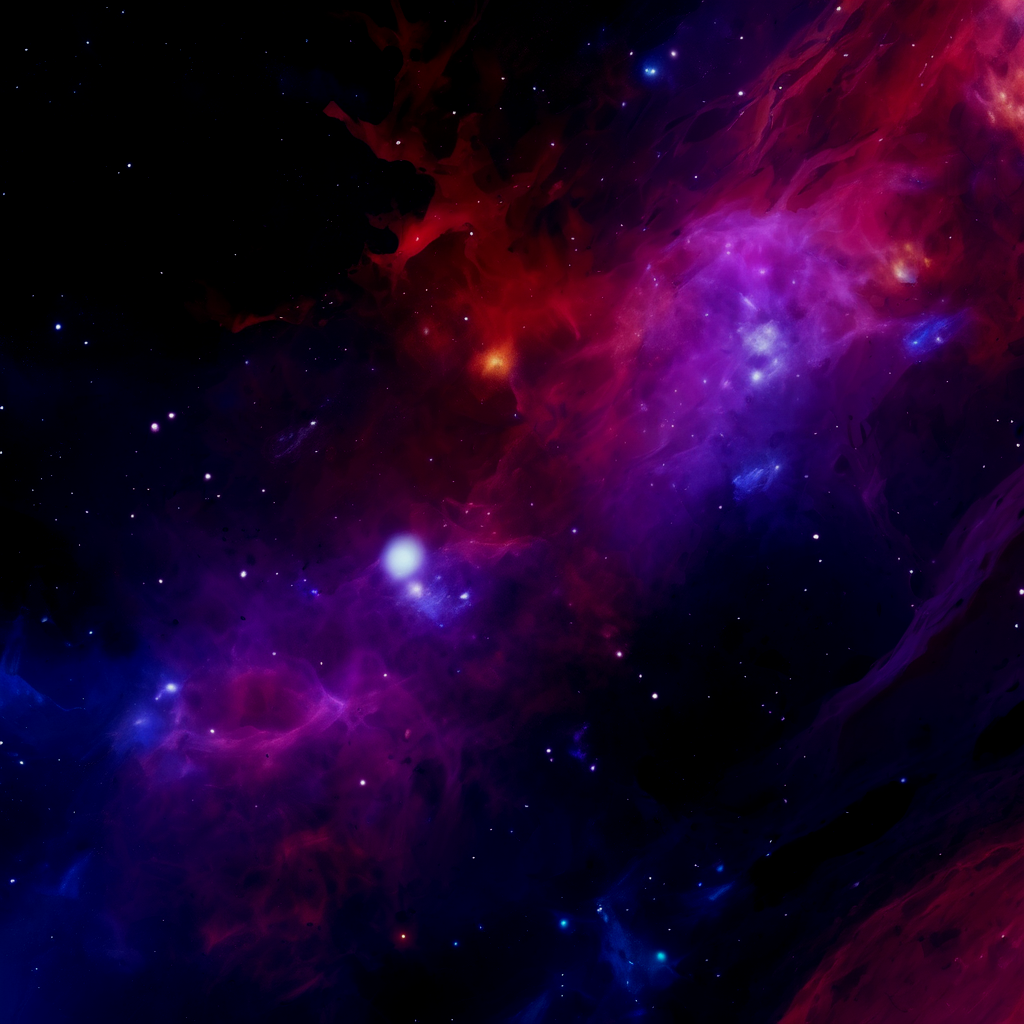
\includegraphics[height=\paperheight,width=\paperwidth]{fondo}};
  \end{tikzpicture}
}%
\usetikzlibrary{arrows.meta, decorations.pathmorphing,positioning,trees}

\lstset{
    basicstyle=\ttfamily\small,
    breaklines=true,
    backgroundcolor=\color{black!98},
    keywordstyle=\color{Magenta},
    commentstyle=\color{AntiqueWhite},
    stringstyle=\color{Yellow!80!white},
    showstringspaces=false,
    frame=single,
    rulecolor=\color{mypurple},
    frameround=tttt,
    escapeinside={\%*}{*)}
}

\makeatletter
% Set victor mono as default ttfont
\newtcolorbox{blur}[1][]{%
  #1,
  enhanced,
  remember,
  breakable, % Already enabled (good!)
  frame hidden,
  interior hidden,
  fonttitle=\bfseries\centering, 
  fontupper=\rmfamily\selectfont,
  coltext=white,
  underlay={
    \begin{tcbclipframe}
      \begin{scope}[inner sep=0pt,remember picture,overlay]
        \fill[white] (frame.south west) rectangle (frame.north east); % Changed to `frame` (not `current page`)
        \node[opacity=1] at (frame.center) {
\includegraphics[height=\paperheight, width=\paperwidth]{blured}};
      \end{scope}
    \end{tcbclipframe}
  }
}
\makeatother
%%%%%%%%%%%%%%%%%%%%%%%%%%%%%%%%%%%%%%%%%%%%%%%%%%%%%%%%%%%%%%%%%%%%%%%%
\newcommand{\separador}[1]{
  \vskip-4pt
  \begin{center}
    \rule{0.9\linewidth}{#1}
  \end{center}
}

\lstset{
  basicstyle=\ttfamily,
  showstringspaces=false,
  breaklines=true
}

\newcommand{\transparencia}[1]{%
  \begin{frame}
    \begin{blur}
      #1
    \end{blur}
  \end{frame}
}

% set bibliography background for text to be legible despite the background

\usepackage{etoolbox}
\newcommand{\setupblurbibliography}{%
  \pretocmd{\frametitle}{\blurbackground}{}{}%
  \setbeamertemplate{bibliography item}{\color{LimeGreen!80!White}\insertbiblabel}%
  \setbeamercolor{bibliography entry author}{fg=AntiqueWhite}%
  \setbeamercolor{bibliography entry title}{fg=Yellow!80!White}%
  \setbeamercolor{bibliography entry location}{fg=AntiqueWhite}%
  \setbeamercolor{bibliography entry note}{fg=AntiqueWhite}%
  \setbeamercolor{bibliography entry url}{fg=Magenta}%
}

\newtcblisting{beamerlst}[1][]{
    enhanced,
    breakable,
    listing only,
    listing options={
        style=beamerlisting,
        language=Python, % Default language
        #1
    },
    colback=black!85, % Matches your theme
    colframe=mypurple, % Your purple color
    fontupper=\ttfamily\small,
    arc=3mm, % Rounded corners
    boxrule=1pt,
    % Blur effect (optional):
    underlay={
        \begin{tcbclipframe}
        \fill[black!90] (frame.south west) rectangle (frame.north east);
        \node[opacity=0.6] at (frame.center) 
            {
\includegraphics[width=\linewidth]{blured}};
        \end{tcbclipframe}
    }
}

% Supporting style definition
\lstdefinestyle{beamerlisting}{
    basicstyle=\ttfamily\footnotesize\color{white},
    keywordstyle=\color{Magenta},
    commentstyle=\color{AntiqueWhite},
    stringstyle=\color{Yellow!80!white},
    showstringspaces=false,
    breaklines=true,
    tabsize=2
}

\newcommand{\codebox}[2][]{%
    \begin{tcolorbox}[
        enhanced,
        colback=black!85,
        colframe=mypurple,
        arc=3mm,
        boxrule=1pt,
        #1
    ]
    \lstinputlisting{#2}
    \end{tcolorbox}%
}

% Smart blur background that works with frame breaks
\newcommand{\blurbackground}{%
  \begin{tikzpicture}[remember picture,overlay]
    % Calculate content area with margins
    \path ([xshift=1cm,yshift=-1cm]current page.north west) coordinate (top left);
    \path ([xshift=-1cm,yshift=1cm]current page.south east) coordinate (bottom right);
    
    % Frosted glass effect
    \fill[black!85,opacity=0.92] (top left) rectangle (bottom right);
    \node[opacity=0.8] at (current page.center) 
      {
\includegraphics[width=\paperwidth-2cm,height=\paperheight-2cm]{blured}};
  \end{tikzpicture}%
}


\includeonly{01.-EvolutionaryComputing}

\bibliography{bibliografia}
\nocite{*}


\author{%
Brandon Marquez Salazar
}
\title{%
  Evolutionary computing
}
\begin{document}
\maketitle
%!TeX root = ProgramaciónEvolutiva.tex
\justifying

  \section*{Introduction}
  \begin{frame}{Introduction}
    \begin{blur}

      \onslide<1,4>
      Evolutionary programming is part of evolutionary algorithms.

      \onslide<2,4>
      The concept of EAs comes from the study of what's called
      \textbf{complex adaptive systems}. 

      \onslide<3,4>
      Its first algorithmic implementation can be traced back to
      Lawrence and David Fogel's work.

    \end{blur}
  \end{frame}


  \begin{frame}{Basic evolutionary process}
  \begin{blur}
    \begin{itemize}
      \item One or more populations of \textbf{individuals competing} for
      limited resources.
      \item The notions of \textbf{dynamically changing} populations due
      to birth and death of individuals.
      \item A concept of \textbf{fitness} which reflects the ability of
      an individual to survive and reproduce.
      \item A concept of \textbf{variational inheritance}: offspring
      closely resemble their parents but are not identical.
    \end{itemize}
  \end{blur}
  \end{frame}

  \begin{frame}{}
  \begin{blur}
    \onslide<1,3>
    Evolutionary algorithms are useful for problem solving due to its
    \textit{complex adaptive behaviour} emulation. Not so different from
    how humans search for solutions to any problem:

    \onslide<2,3>
    \begin{itemize}
      \item Formulating solutions,
      \item then \textbf{evaluating} them:
      \item the best ones are used, the less useful ones are usually
      \textbf{discarded} and
      \item some of them are \textbf{\itshape mutated} or
      \textbf{\itshape recombined} to create new ones, maybe better.
    \end{itemize}
  \end{blur}
  \end{frame}

  \begin{frame}{Evolutionary programming}
  \begin{blur}
    Fogel proposed modeling individuals as finite state machines.

    Also, he proposed sexual and asexual reproduction of individuals
    in the algorithm.

    The program should start with a N number of initial individuals;
    and the next generation is determined by combining new individuals
    into a 2N population, raking them and selecting the best N
    individuals.
  \end{blur}
  \end{frame}

  \begin{frame}{Problem solving}
  \begin{blur}
    \onslide*<1> {
        Since simple rules could demonstrate complex behaviour and some
        sort of intelligent exploration in a space of possible solutions,
        we can use EAs to solve problems.
    }

    \onslide*<2> {
      Each problem should be modeled in order to find
      \begin{itemize}
        \item An individual definition that satifies the problem's
        solution space characterization.
        \item A fitness function that describes correctly our problem's
        behaviour.
        \item A \textbf{variation operator} that generates new
        individuals from existing ones.
        \item A \textbf{selection operator} that selects the best
        individuals from the population.
      \end{itemize}
    }
    \onslide*<3>{
      This can be applied, for example , not only to simple problems (like
      function maximization/minimization) but to more complex ones like
      ANN's weights tuning, scheduling, energy consumption optimization, etc.
    }
  \end{blur}
  \end{frame}


%!TeX root = ProgramaciónEvolutiva.tex
\section*{Evolutionary computing}
\begin{frame}
  \begin{blur}
    \begin{center}
      {\LARGE Evolutionary programming}
    \end{center}
  \end{blur}
\end{frame}

\begin{frame}
  \begin{blur}

    Following what John R. Koza said in his essay Human-Competitive Machine
    Intelligence \cite{PEADNAS2003}, points that evolutionary algorithms can be
    used in order to make a computer program to solve (approximately)
    a problem.

  \end{blur}
\end{frame}

\begin{frame}[fragile,allowframebreaks]{The problem, the model and the solution}
  \begin{blur}

  Think about a problem. Usually, to solve some problem, we can solve it
  using tools that are already available. For example, if we want to know
  the position of a particle at a certain time in an uniform rectilinear
  motion problem, we can solve it by a simple equation.
  \begin{figure}[!ht]
    \begin{center}
    \begin{tikzpicture}[>=Stealth, font=\sffamily\small]

      % Experiment surface
      \draw[thick, fill=black!90] (0,0) rectangle (8,1);
      \draw[<->] (0,-0.5) -- (8,-0.5) node[right]{$X$};

      %Equation $X_f(t) = X_0 + V_0 t$
      \draw node at (4,1.8) {$X_f(t) = X_0 + V_0 t$};

      % Moving object
      \filldraw[fill=blue!30, draw=blue!50!black] (1,0.5) rectangle node[black]{$m$} (2,1.2);

      % Force arrow
      \draw[->, Yellow, thick] (2,0.85) -- node[above]{$\vec{V}$} (3.5,0.85);

      % Measurement markers
      \foreach \x in {0,2,4,6,8} {
        \draw (\x,0) -- (\x,-0.15) node[below]{$\x$};
      }

    %% Motion trace
    %\draw[decorate, decoration={snake, amplitude=0.5mm, segment length=2mm}] 
    %(2,1.4) -- node[above]{Motion trace} (6,1.4);

    % Coordinate axes
    %\draw[->] (0.2,0.2) -- (0.2,1.2) node[right]{$y$};
    %\draw[->] (0.2,0.2) -- (1.2,0.2) node[above]{$x$};

    \end{tikzpicture}
    \end{center}
    \caption{Uniform rectilinear motion [Deepseek]}
  \end{figure}

  \end{blur}
  \begin{blur}
    And we can call it a simulation, which is the most common thing, and
    easiest thing to do with a computer.
  \end{blur}
  
  \begin{beamerlst}[language=python]
class Particle:
  def __init__(self, x0, v0):
    self.x0 = x0
    self.v0 = v0

  def simulate(self, t):
    return self.x0 + self.v0 * t

  def __repr__(self):
    return f'Particle(x0={self.x0}, v0={self.v0})'
     
if __name__ == '__main__':
  p = Particle(0, 10)
  print(p.simulate(10))
  \end{beamerlst}
  \begin{center} \rule{0.9\linewidth}{0.4pt} \end{center}

  \vfill

  \begin{beamerlst}
  %% Output as in a python shell
  >_ python particle.py
  100
  \end{beamerlst}

  \vfill

  \begin{center} \rule{0.9\linewidth}{0.4pt} \end{center}
  \newpage

  \begin{blur}
    But now, what happens if we haven't an equation or an algorithm to solve
    the problem? If have data and we need to know how it's behaving? What if
    we need to predict it's behaviour? Maybe some nonlinear phenomena,
    a signal, classification, or something not so intuitive as common
    problems? 
  \end{blur}
  
  \begin{blur}
    Here is where modeling comes in \cite{Eiben2015}. And here is where genetic programming
    started to gain relevance.
  \end{blur}
  

\end{frame}

\begin{frame}[allowframebreaks]{Modeling}

    \begin{blur}
      Genetic programming is an implementation of genetic algorithms where
      the individuals are programs which are intended to solve a given
      problem

      \begin{figure} [!ht]
        \begin{center}
          \begin{tikzpicture}[
            x=0.4cm, y=0.4cm,
            level distance=1.4cm,
            level 1/.style={sibling distance=2cm},
            level 2/.style={sibling distance=1.5cm},
            every node/.style={
              draw, 
              circle, 
              fill=cyan!30!black, 
              text=white, 
              minimum size=0.8cm,
              font=\small
            },
            edge from parent/.style={
              draw, 
              ->, 
              >=stealth, 
              shorten >=2pt, 
              thick, 
              cyan!50
            }
            ]

          % Root node (+)
            \node {\textcolor{Yellow}{$+$}}
            child {
                  % Left subtree (x^2)
              node {\textcolor{Yellow}{$\times$}}
              child {
                node {$x$}
              }
              child {
                node {$x$}
              }
            }
            child {
                  % Right subtree (x)
              node {$x$}
            }
            ;
          \end{tikzpicture}
        \end{center}
        \caption{Genetic programming solution tree for $x^2 + x$ [Deepseek]}
      \end{figure}
    \end{blur}


    \section{Ejemplos}
    \begin{blur}

      Aquí se muestra un ejemplo de la implementación de un algoritmo genético para
      programación genética utilizando el framework DEAP \cite{DEAPGENETIC}.

      \begin{itemize}
        \item \href{run:./Ejemplo/DEAP-GP.html} {\underline{Ejemplo HTML}}
        \item \href{run:./Ejemplo/DEAP-GP.pdf}   {\underline{Ejemplo PDF}}
        \item \href{run:./Ejemplo/DEAP-GP.ipynb}{\underline{Ejemplo Jupyter}}
        \item \href{run:./Ejemplo/DEAP_GP.py}   {\underline{Ejemplo Python}}
    \end{itemize}

    \end{blur}

\end{frame}


% Beamer bibliography

\begin{frame}[allowframebreaks]{References}
  \printbibliography[heading=none]
\end{frame}

\end{document}
